%%%%%%%%%%%%%%%%%%%%%%%%%%%%%%%%%%%%%%%%%%%%%%%%%%%%%%%%%%%%%%%%%%%%%%%%%%%%%%%%
%2345678901234567890123456789012345678901234567890123456789012345678901234567890
%        1         2         3         4         5         6         7         8

\documentclass[letterpaper, 10 pt, conference]{ieeeconf}  % Comment this line out
                                                          % if you need a4paper
%\documentclass[a4paper, 10pt, conference]{ieeeconf}      % Use this line for a4
                                                          % paper

\IEEEoverridecommandlockouts                              % This command is only
                                                          % needed if you want to
                                                          % use the \thanks command
\overrideIEEEmargins
% See the \addtolength command later in the file to balance the column lengths
% on the last page of the document

\usepackage{graphicx,graphics}
\usepackage{amssymb,amsmath}
\usepackage{amsfonts}
\usepackage{calrsfs} % for calligraphic font in math mode
\usepackage{subfigure}
\usepackage{url}
\usepackage{color}

% The following packages can be found on http:\\www.ctan.org
%\usepackage{graphics} % for pdf, bitmapped graphics files
%\usepackage{epsfig} % for postscript graphics files
%\usepackage{mathptmx} % assumes new font selection scheme installed
%\usepackage{times} % assumes new font selection scheme installed
%\usepackage{amsmath} % assumes amsmath package installed
%\usepackage{amssymb}  % assumes amsmath package installed

\title{\LARGE \bf
Counter UAS using a Formation Controlled Dragnet
}


\author{Skyler Tolman and Randal W. Beard$^{1}$% <-this % stops a space
\thanks{*This work was not supported by any organization}% <-this % stops a space
\thanks{$^{1}$S. Tolman is a research assistant, and R. Beard is with the Department of Electrical and Computer Engineering, Brigham Young University, Provo, UT 84602, OH 45435, USA.  
        {\tt\small skyler237 at gmail.com}, 
        {\tt\small beard at byu.edu}}%
}


\begin{document}

\maketitle
\thispagestyle{empty}
\pagestyle{empty}


%%%%%%%%%%%%%%%%%%%%%%%%%%%%%%%%%%%%%%%%%%%%%%%%%%%%%%%%%%%%%%%%%%%%%%%%%%%%%%%%
\begin{abstract}

blah, blah...

\end{abstract}


%%%%%%%%%%%%%%%%%%%%%%%%%%%%%%%%%%%%%%%%%%%%%%%%%%%%%%%%%%%%%%%%%%%%%%%%%%%%%%%%
\section{INTRODUCTION}

- [motivation for counter UAS]

- [list some of the possible options and their strengths and weaknesses]

- [Describe our approach at a high level, i.e, a team of UAS towing a net.  Maybe add a figure to illustrate.]

- [Talk a little about formation control - RWB to do this]

- [Talk about different intercept strategies]	

- [Comparing existing intercept strategies used for defense against a new one - Adaptive Radius]

- [situation is 4 multirotors holding a net, defending a central location, defending against one incoming multirotor]

%%%%%%%%%%%%%%%%%%%%%%%%%%%%%%%%%%%%%%%%%%%%%%%%%%%%%%%%%%%%%%%%%%%%%%%%%%%%%%%%
\section{PROBLEM STATEMENT}

This paper is primarily focused on the algorithm used for interception. We assume some idealities and do not address every aspect of the full system, but we use the same assumptions and parameters for each intercept strategy. This allows us to make a reasonable comparison of the different intercept approaches, isolated from other aspects of the scenario.

{\em Terminology:} We will refer to the four multirotor and net system as “the fleet” and refer to the incoming multirotor UAV as “the intruder.” The central location which the fleet is defending will be referred to as the “center of defense.”


{\em Assumptions:}
\begin{itemize}
\item We assume no wind. 
\item We disregard any dynamics that would be introduced by a net carried by the fleet UAS and treat them as dynamically independent vehicles and do not address formation control. 
\item We assume, unless otherwise stated, that the fleet of UAS and the intruder UAV are similar in speed and capability.
\item We allow aggressive maneuvers for the intruder, but do not model any obstacle avoidance behavior.
\item We do not simulate sensors or estimation of states, but use global truth values for all position and velocity measurements.
\end{itemize}

%%%%%%%%%%%%%%%%%%%%%%%%%%%%%%%%%%%%%%%%%%%%%%%%%%%%%%%%%%%%%%%%%%%%%%%%%%%%%%%%
\section{INTERCEPT STRATEGIES}

%----------------------------------------
\subsection{ProNav (Proportional Navigation)}
Proportional Navigation (ProNav) is a common interception scheme used in missile guidance systems. Here we will use a 3-D implementation of ProNav focused on UAV control [ProNav citation here]. The algorithm produces a desired acceleration perpendicular to the movement of the aircraft which is proportional to the line of sight vector and the closing velocity. The equations used to implement this method are listed below:


Let the position of the fleet be the central location of the net carried by the fleet UAS and be represented by \(p_F\). Let the position of the intruder be represented as \(p_I\).

Define \(\ell = p_I - p_F\) and \(\dot{\ell} = \dot{p_I} - \dot{p_F}\). Let $L = \|\ell\|$.

\[
	a_F = N\Omega_\perp \times \mu v_F
\]
where
\[
	\Omega_\perp = \frac{\ell}{L} \times \frac{\dot{\ell}}{L}
\]
\[
	\mu = \frac{\|\dot{\ell}\|}{\|v_F\|}
\]
and where $a_F$ is the commanded acceleration for the fleet.

Pros and Cons: ProNav is a minimal cost algorithm that is efficient for missile guidance, but it is based upon the assumption that the interceptor has a much higher velocity than the target. ProNav also is not very good at switching between intercepting and oncoming target and following a target. This can be problemsome if the intruder alternates between moving toward and away from the center of defense.

Example of an equation:
\[
\dot{r} = \sin\phi
\]

Here is how to do a figure
\begin{figure}[hbt]
  \centering
  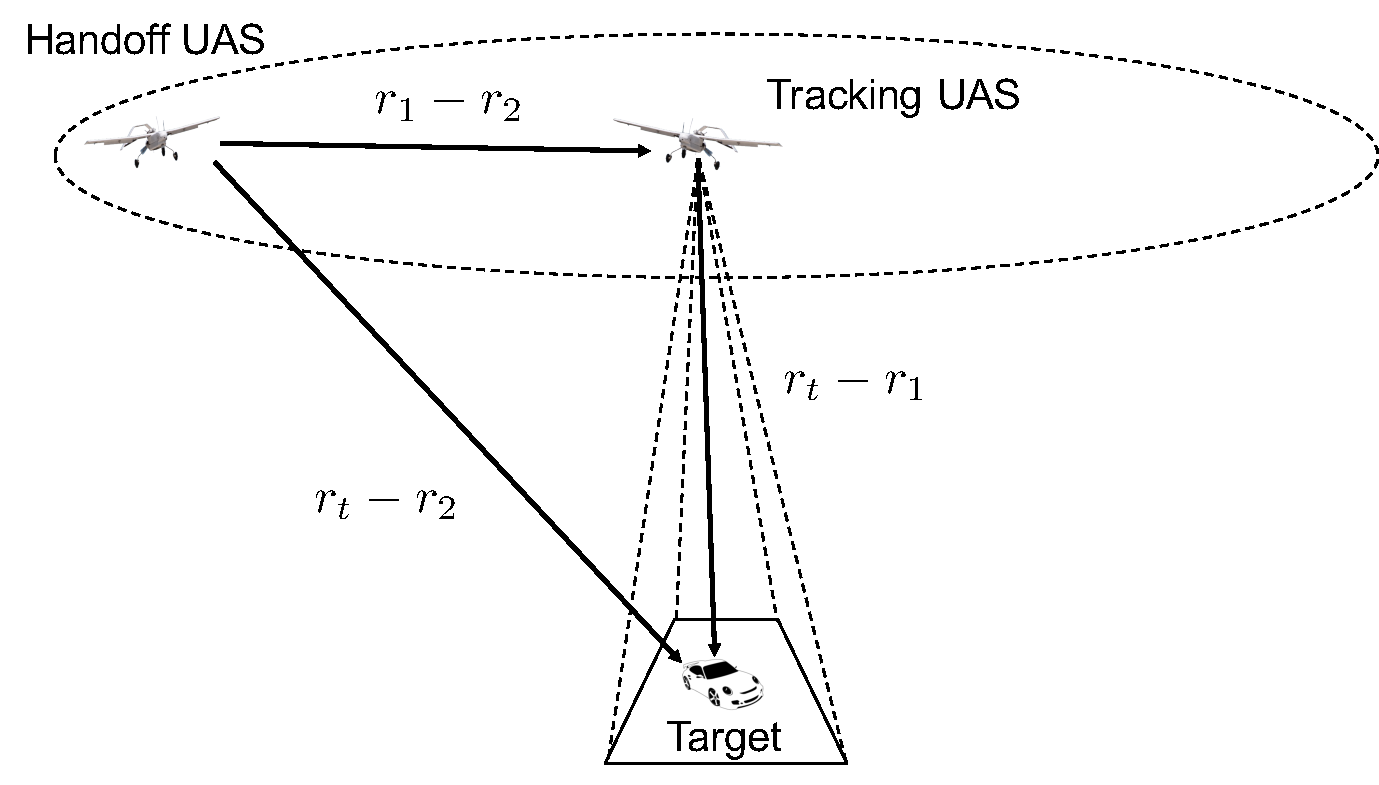
\includegraphics[width=0.45\textwidth]{figures/scenario}
  \caption{Caption goes here.}
  \label{fig:label}
\end{figure}

Here is how to cite something~\cite{Siouris04}.

%----------------------------------------
\subsection{Target-predictive Smoothed Waypoint Path}
This algorithm attempts to predict the future position of the intruder and create a 3rd degree polynomial path to the optimal intercept point. 

The digital implementation of this algorithm utilizes a binary search to calculate the optimal path that will allow the fleet to intercept the intruder at an optimal time. This is the basic algorithm used:

The algorithm below was adapted from a ball intercept algorithm used for robot soccer:
\newline

The algorithm uses the following functions
\newline

$p_t^+$ = \textbf{targetPredict}($t^+$): Returns the predicted target position at time $t^+$ into the future

$P$ = \textbf{planPath}($p_1, p_2, h$): Plans a waypoint path from point $p_1$ to $p_2$, such that the direction of the final leg of the path is identical to $h$. 

$L$ = \textbf{pathLength}($P$): Returns the path length of $P$.
\newline

We can predict the path length to the predicted target location as being

\[
L = \textnormal{pathLength}(\textnormal{planPath}(z, \textnormal{targetPredict}(t^+),h))
\],

where $z$ is the current location of the UAS fleet. The time it takes the UAS to traverse this path with velocity $v$ is given by

\[
T(t^+) = \frac{\textnormal{pathLength}(\textnormal{planPath}(z, \textnormal{targetPredict}(t^+),h))}{v}
\]

Define the function

\[
g(T) = vT - \textnormal{pathLength}(\textnormal{planPath}(z, \textnormal{targetPredict}(T),h))
\]

The ideal intercept time is the smallest $T^*$ that satisfies the equation $g(T^*) = 0$. The ideal intercept time can be found using a binary search algorithm. Note that $g(0) < 0$, and that for some $T > 0$, we are guaranteed that $g(T) > 0$. Therefore, the following algorithm will quickly converge to $T*$.
\newline


\begin{enumerate}
\item 
\end{enumerate}
\textbf{Bisection Search Algorithm}

\textbf{Step 1:} Set $T = 0$, $T_1 = 0$.

\textbf{Step 2:} Incrementally increase $T$ until $g(T) > 0$. Set $T_2 = T$.

\textbf{Step 3:} While \(\|g(\frac{T_1 + T_2}{2} > \epsilon\) if 

[ Robot Soccer Notes citation (?) ]

Pros and Cons: This approach is efficient for intercepting predictable targets, but it is ineffective against targets with more predictable or aggressive paths. In many cases, this algorithm performed the worst out of the three because the target prediction was ineffective and misleading most of the time. Perhaps, it would be advantageous to revisit this option in the future using a more robust prediction scheme.


%----------------------------------------
\subsection{Adaptive Radius Optimal Defense}
	Adaptive Radius Optimal Defense (AROD) is designed to optimize interception in a defensive situation where an offensive scheme is not necessary. It is takes into account an inherent control delay between the fleet and an intruding UAV. 
	
    In this strategy, the fleet deploys to a maximum radius and tracks the intruder position on that radius. The radius on which the fleet resides is dynamically increased based on the chance the fleet has to capture the intruder and is decreased based on how likely we are to miss the intruder. By adapting the fleet radius in this way, we can effectively increase the maximum allowable reaction time in order to respond to a maneuver performed by the intruder.
	
    The algorithm and equations are explained in more detail below:

[Insert equations and algorithm]

Pros and Cons: The main advantage to this approach is that the fleet can focus its energy and efforts on defending a central location and minimizing the chance of missing the target. As a direct result, one disadvantage of this approach is that it is not offensively aggressive. It also often takes longer to intercept and the interception occurs at a radius closer to the center. But these are just a couple tradeoffs of maximizing the probability of a successful interception.

%%%%%%%%%%%%%%%%%%%%%%%%%%%%%%%%%%%%%%%%%%%%%%%%%%%%%%%%%%%%%%%%%%%%%%%%%%%%%%%%
\section{SIMULATION RESULTS}

Varying number of maneuvers

Varying proximity before maneuvers

Varying intruder max velocity vs. fleet max velocity

Varying net size

%%%%%%%%%%%%%%%%%%%%%%%%%%%%%%%%%%%%%%%%%%%%%%%%%%%%%%%%%%%%%%%%%%%%%%%%%%%%%%%%
\section{CONCLUSION}

%%%%%%%%%%%%%%%%%%%%%%%%%%%%%%%%%%%%%%%%%%%%%%%%%%%%%%%%%%%%%%%%%%%%%%%%%%%%%%%%


\addtolength{\textheight}{-12cm}   % This command serves to balance the column lengths
                                  % on the last page of the document manually. It shortens
                                  % the textheight of the last page by a suitable amount.
                                  % This command does not take effect until the next page
                                  % so it should come on the page before the last. Make
                                  % sure that you do not shorten the textheight too much.

\section*{ACKNOWLEDGMENT}
This research was conducted in the Center for Unmanned Aircraft Systems (C-UAS) with
support from the National Science Foundation I/UCRC program grant number IIP-1161036 and
C-UAS Industry Advisory Board members.


%%%%%%%%%%%%%%%%%%%%%%%%%%%%%%%%%%%%%%%%%%%%%%%%%%%%%%%%%%%%%%%%%%%%%%%%%%%%%%%%
\bibliographystyle{IEEEtran}
\bibliography{library}

\end{document}
